\section{Добавление аккаунта эл.почты на планшет}
Перед началом настройки аккаунта электронной почты торговый представитель должен убедиться, что планшет  подключён к сети интернет и заряд планшета достаточен для уверенной работы. У торгового представителя на руках должна быть информация о  его аккаунте (логин и пароль).

Для добавления аккаунта эл.почты необходимо выполнить следующие действия:
\begin{enumerate}[\thesection .1]

 \begin{figure}[H]
 	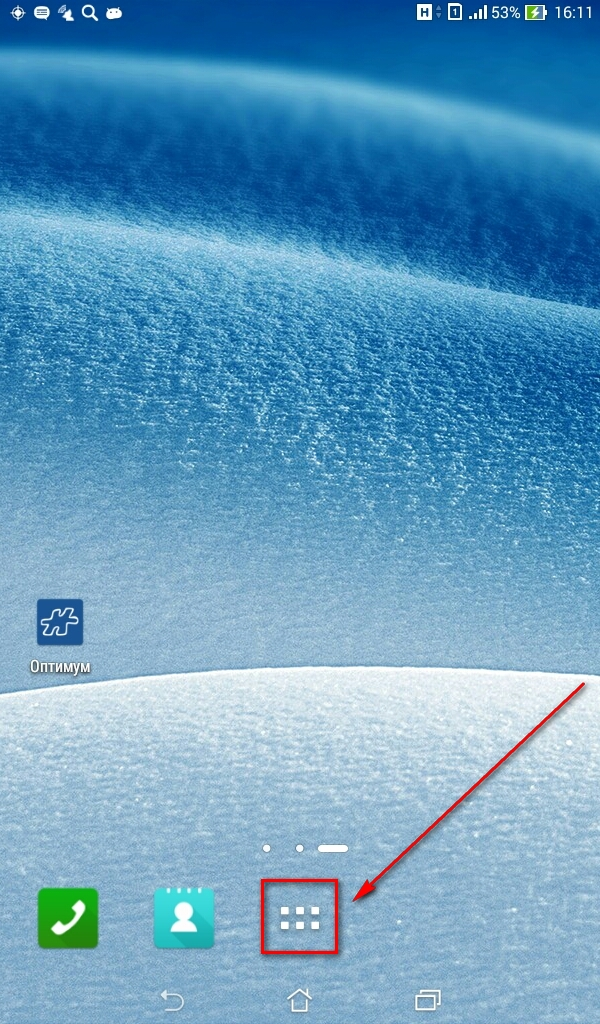
\includegraphics[width=0.3\linewidth]{pic_1.jpg} 
 	\caption{Меню}\label{pic:pic_1}
 \end{figure}
\item  Зайти в меню планшета используя стандартную иконку (рис.\ref{pic:pic_1}): 
\newpage 

\begin{figure}[!h]
	\begin{floatrow}
		\ffigbox{\caption{Настройка}\label{pic:pic_2}}%
		{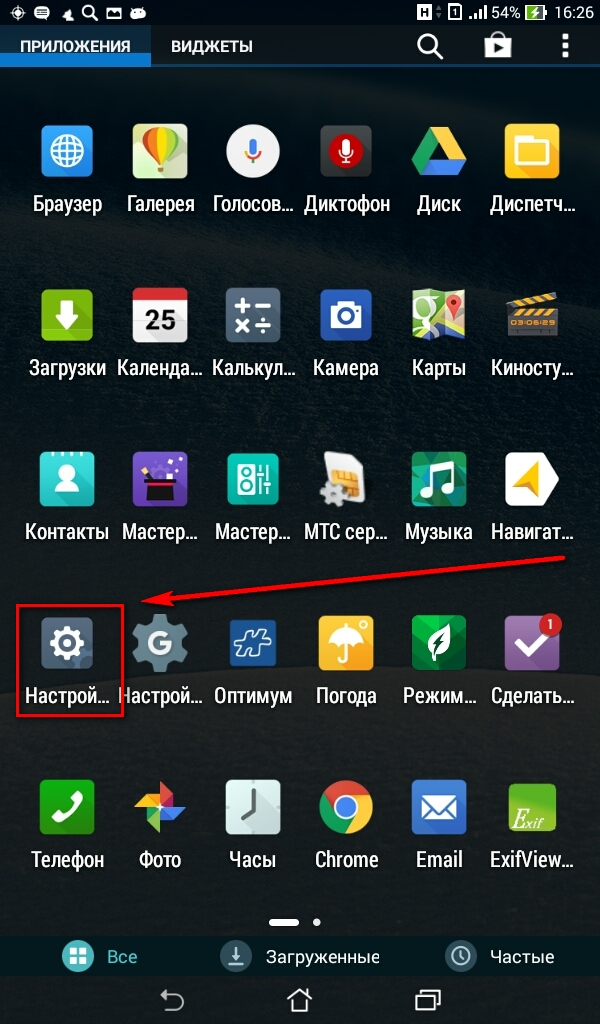
\includegraphics[width=0.58\linewidth]{pic_2.jpg}}
		\ffigbox{\caption{Настройки планшета}\label{pic:pic_3}}%
		{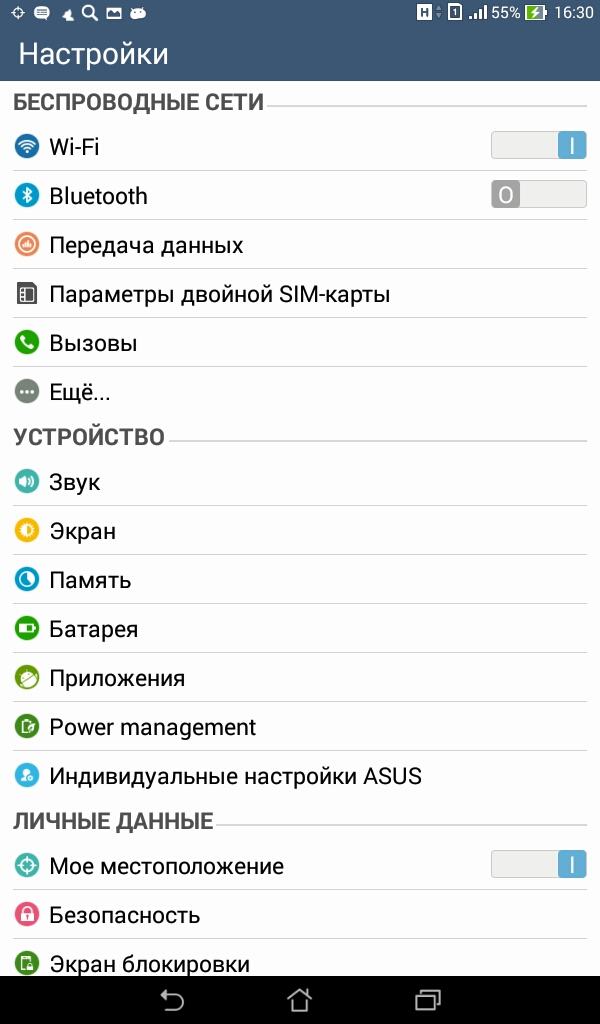
\includegraphics[width=0.58\linewidth]{pic_3.jpg}}         
	\end{floatrow}
\end{figure}
 
\item Выбрать и нажать на значок "Настройка" планшета (рис.\ref{pic:pic_2}):
\item Откроется окно настроек планшета (рис.\ref{pic:pic_3}):
%\newpage 

\begin{figure}[!h]
	\begin{floatrow}
		\ffigbox{\caption{Добавить аккаунт}\label{pic:pic_4}}%
		{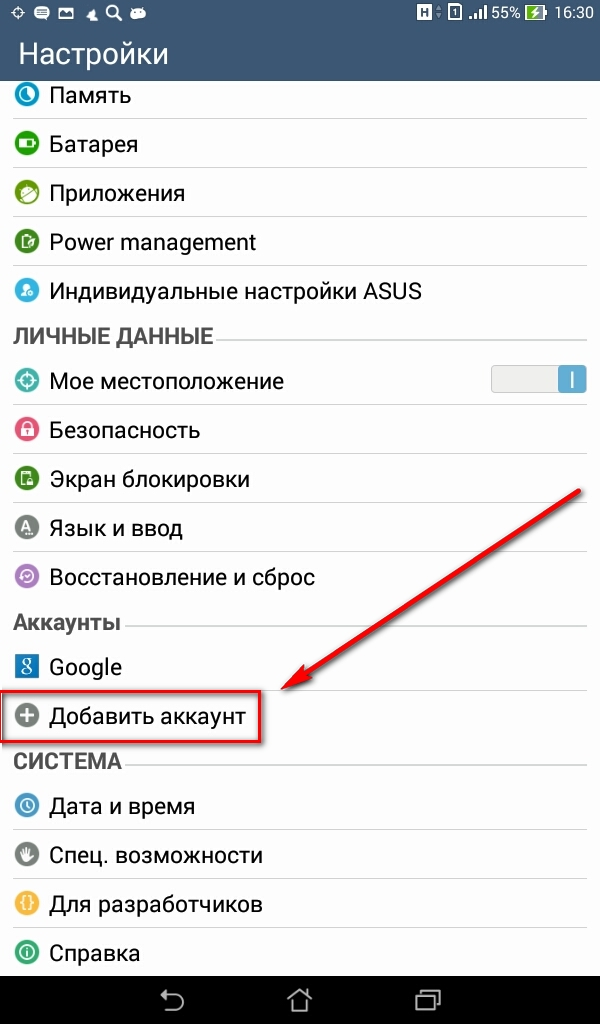
\includegraphics[width=0.58\linewidth]{pic_4.jpg}}
		\ffigbox{\caption{Google}\label{pic:pic_5}}%
		{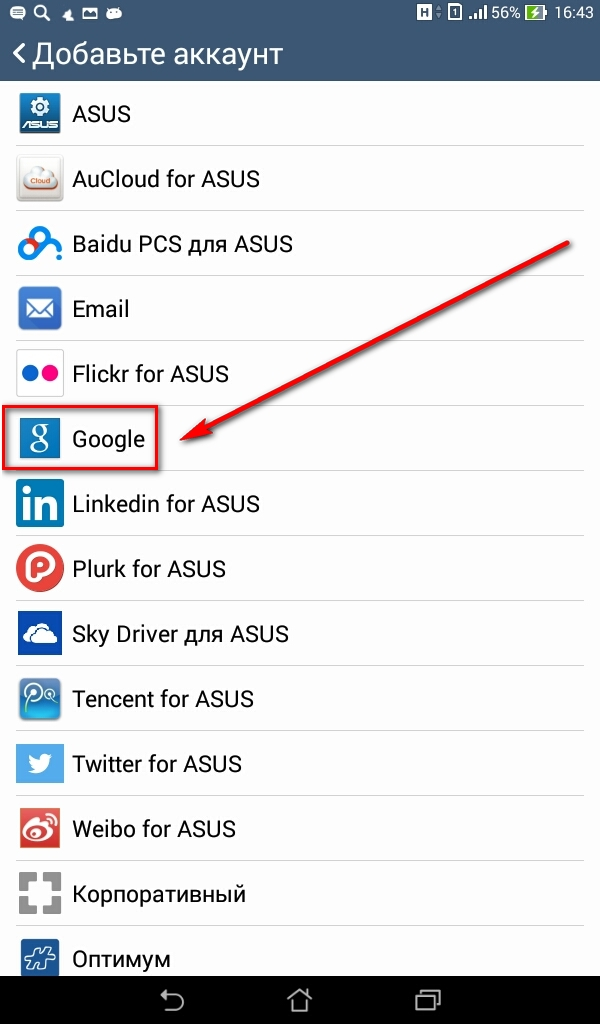
\includegraphics[width=0.58\linewidth]{pic_5.jpg}}         
	\end{floatrow}
\end{figure}
 
\item "Пролистать" список вниз до появления пункта "Добавить аккаунт" (рис.\ref{pic:pic_4}):
\item Выбрать его, затем найти и выбрать "Google" (рис.\ref{pic:pic_5}):

\newpage

\begin{figure}[!h]
	\begin{floatrow}
		\ffigbox{\caption{Существующий аккаунт}\label{pic:pic_6}}%
		{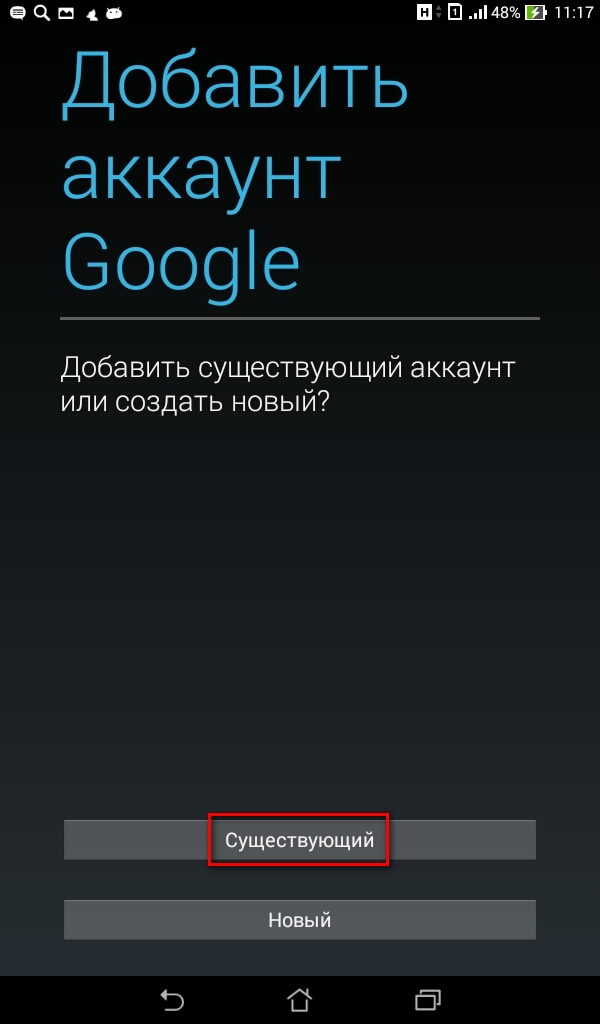
\includegraphics[width=0.58\linewidth]{pic_6.jpg}}
		\ffigbox{\caption{Ввод данных}\label{pic:pic_7_1}}%
		{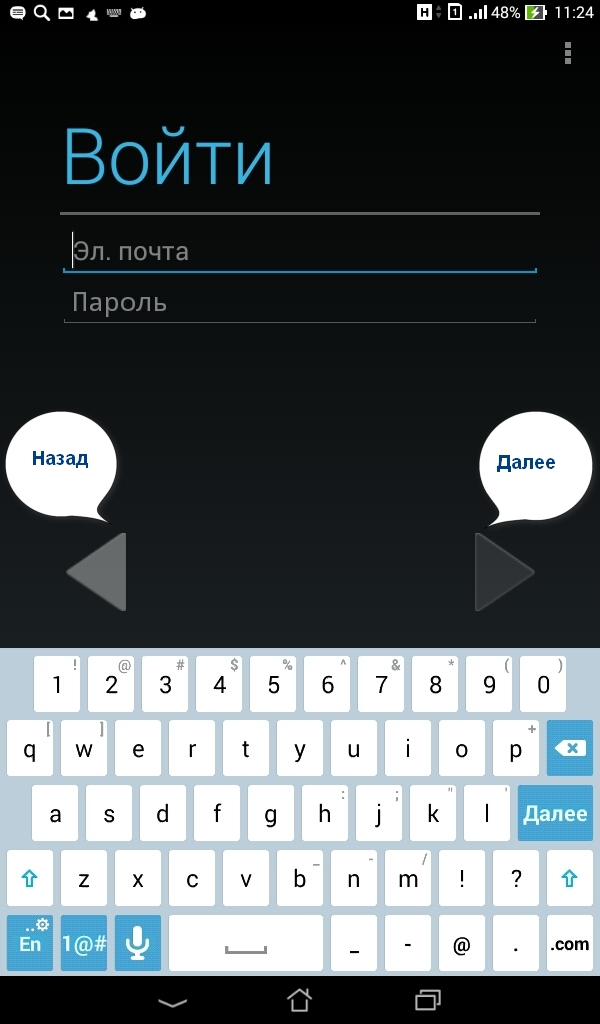
\includegraphics[width=0.58\linewidth]{pic_7_1.jpg}}         
	\end{floatrow}
\end{figure}

\item В открывшемся окне необходимо использовать кнопку "Существующий" (рис.\ref{pic:pic_6}):
\item В следующем появившемся окне необходимо ввести название ящика эл.почты и пароль, их должно выдать ваше руководство(рис.\ref{pic:pic_7_1}):
\item Для навигации по настройкам аккаунта используйте треугольные кнопки "Назад" и "Далее" 
	  	

%\newpage

\begin{figure}[!h]
	\begin{floatrow}
		\ffigbox{\caption{Введённые данные}\label{pic:pic_8}}%
		{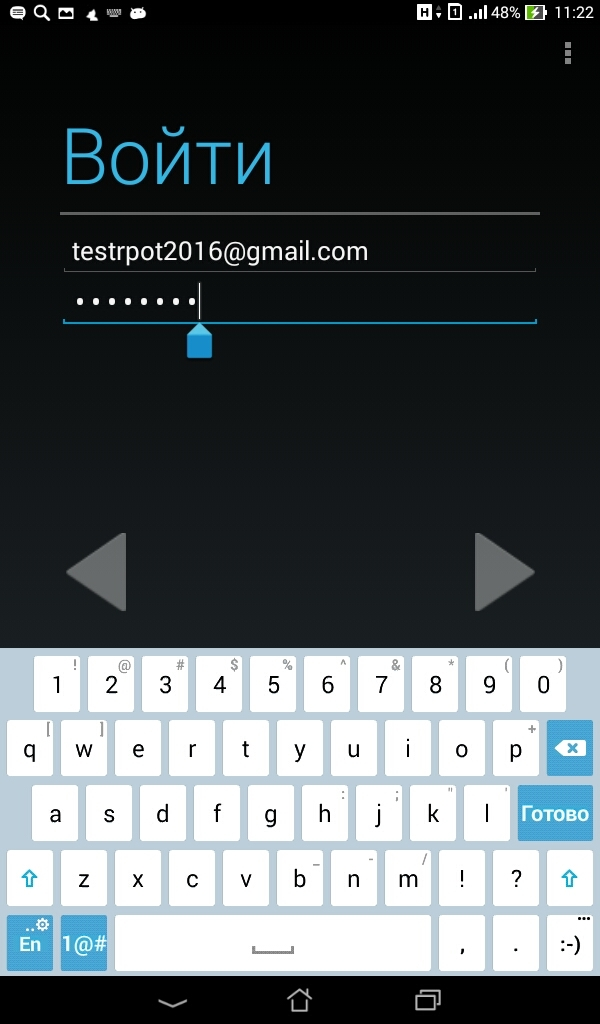
\includegraphics[width=0.58\linewidth]{pic_8.jpg}}
		\ffigbox{\caption{Заполненные данные}\label{pic:pic_9}}%
		{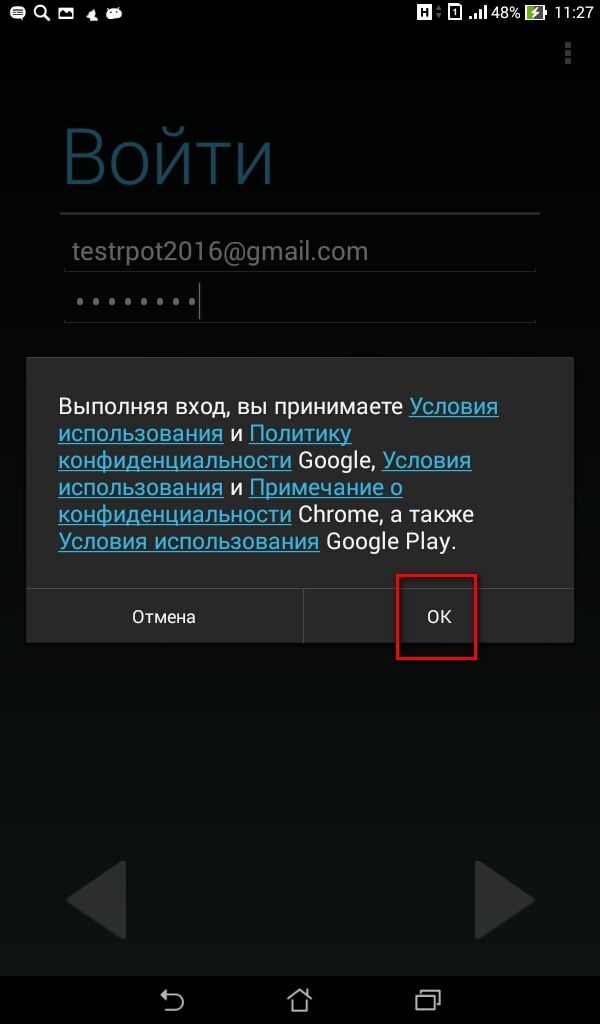
\includegraphics[width=0.58\linewidth]{pic_9.jpg}}         
	\end{floatrow}
\end{figure}

%\item  (рис.\ref{pic:pic_6}):
\item После ввода данных и нажатия стрелки далее, появляется запрос на который нужно ответить "Ок"  (рис.\ref{pic:pic_9}):
 

\newpage
\begin{figure}[H]
 	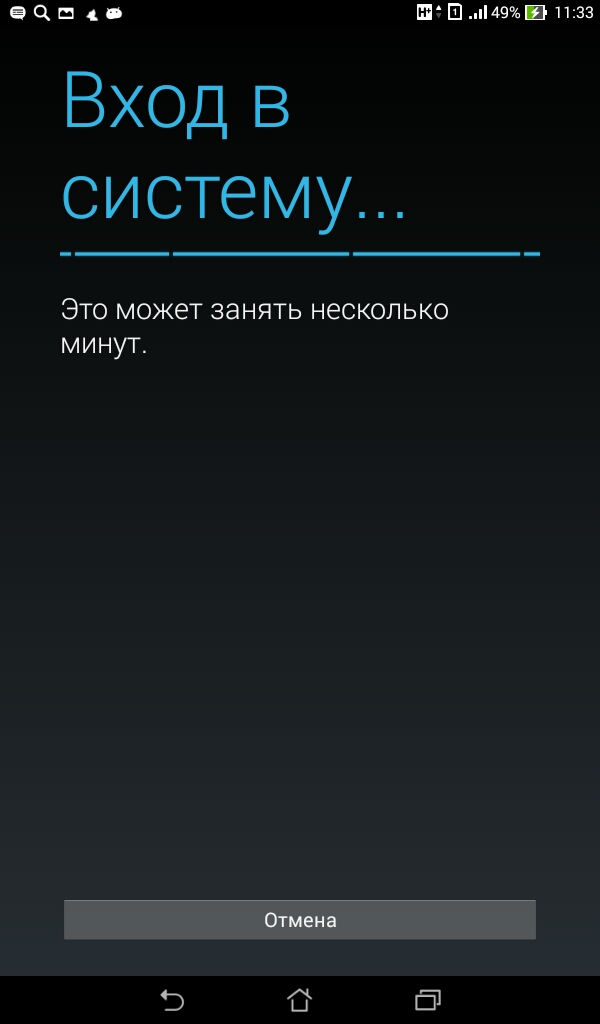
\includegraphics[width=0.3\linewidth]{pic_10.jpg} 
 	\caption{Проверка данных}\label{pic:pic_10}
\end{figure}
\item Далее ожидаем проверки введённых данных (рис.\ref{pic:pic_10}):


\begin{figure}[!h]
	\begin{floatrow}
		\ffigbox{\caption{Запрос на подписки}\label{pic:pic_11}}%
		{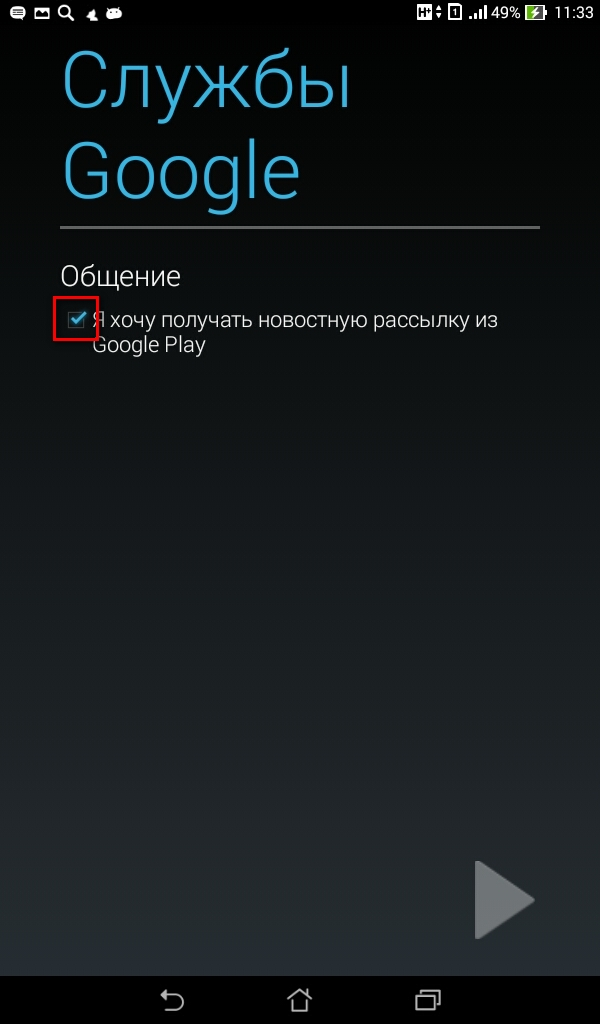
\includegraphics[width=0.58\linewidth]{pic_11.jpg}}
		\ffigbox{\caption{Отказ от подписок}\label{pic:pic_12}}%
		{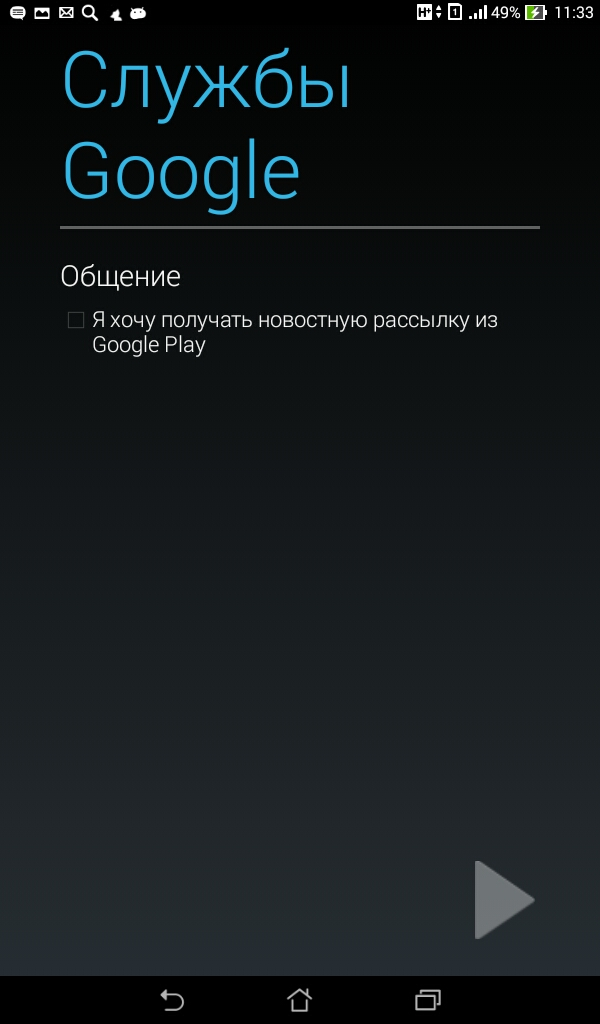
\includegraphics[width=0.58\linewidth]{pic_12.jpg}}         
	\end{floatrow}
\end{figure}

\item Если проверка прошла нормально вы увидите запрос о получении новостных рассылок от Google  (рис.\ref{pic:pic_11}), необходимо снять это галку и нажать далее (рис.\ref{pic:pic_12}):
Если проверка не прошла, то необходимо вернуться к окну ввода эл.почты и пароля и внимательно повторить ввод.  

\newpage
\begin{figure}[H]
	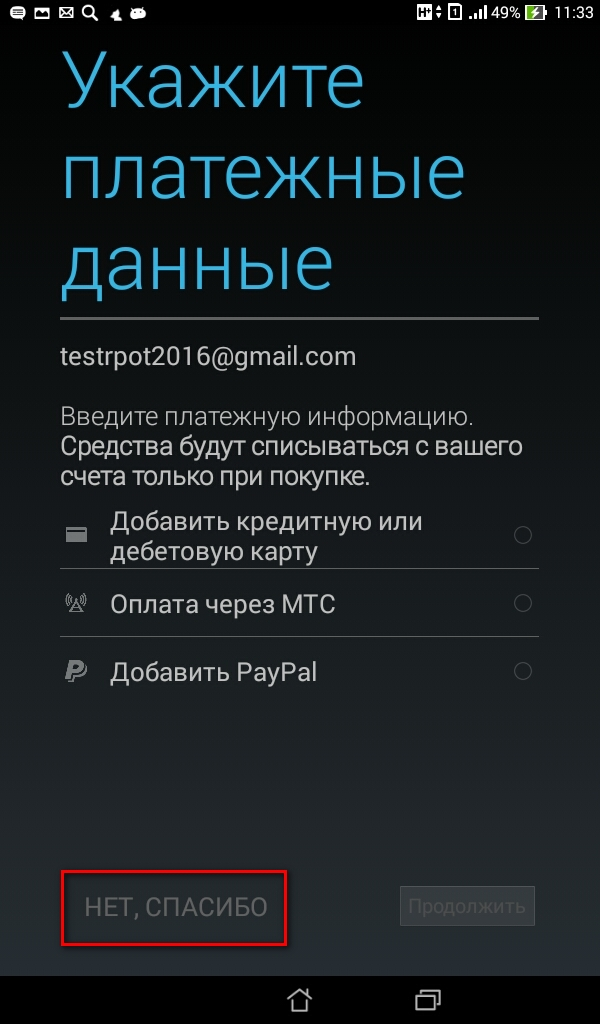
\includegraphics[width=0.3\linewidth]{pic_13.jpg} 
	\caption{Платёжные данные}\label{pic:pic_13}
\end{figure}
\item Затем Google просит указать платёжные данные, выбираем вежливое "Нет, спасибо" (рис.\ref{pic:pic_13}):
  
\begin{figure}[!h]
	\begin{floatrow}
		\ffigbox{\caption{Запрос на синхронизацию}\label{pic:pic_14}}%
		{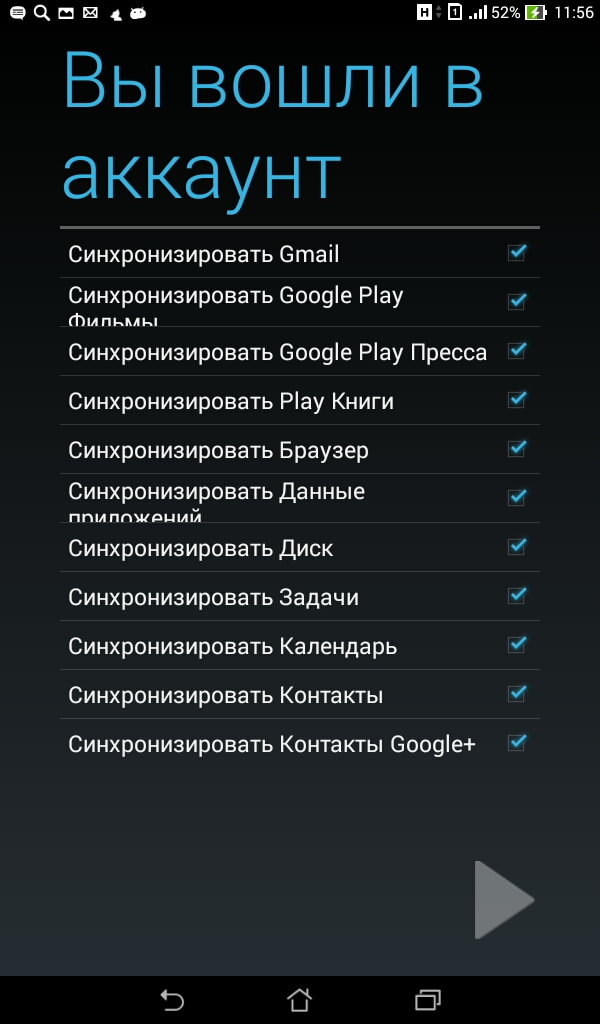
\includegraphics[width=0.58\linewidth]{pic_14.jpg}}
		\ffigbox{\caption{Отказ от синхронизации}\label{pic:pic_15}}%
		{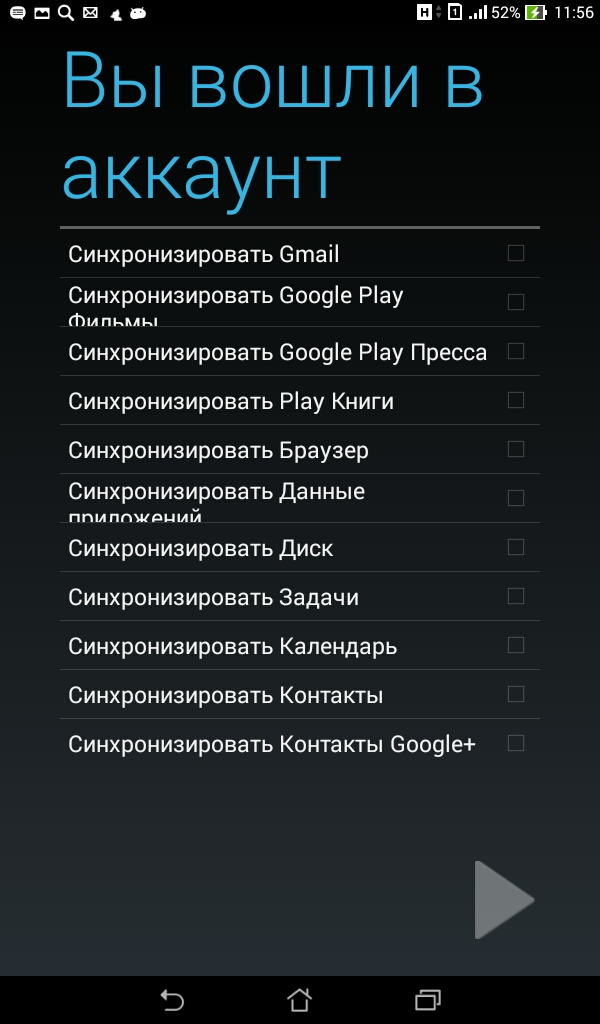
\includegraphics[width=0.58\linewidth]{pic_15.jpg}}         
	\end{floatrow}
\end{figure}

\item На следующем экране Google предлагает настройки синхронизации (рис.\ref{pic:pic_14}), снимаем все галочки и нажимаем далее (рис.\ref{pic:pic_15}), аккаунт заведён, вы снова попадаете в настройки планшета.

\end{enumerate}